\chapter{RELATED WORK}
\label{chp:relatedwork}

In this chapter, studies related to the work presented in this thesis are presented. Firstly, latest trends and studies in the process mining area are explained. Then studies from cross-organizational process mining, which is the main topic of this research, is introduced. Following these, studies related to similarity in process mining is mentioned. Finally, performance and conformance analysis approaches in process mining area are presented. In each section, survey of related studies are aimed to be limited with the subject of this thesis.

\section{State of the Art in Process Mining}
\label{sec:state-of-the-art-in-process-mining}

In this section, important milestones in process mining and current research trends will be presented. Studies in process mining area have roots based on process discovery techniques for software engineering. These original techniques are studied to discover workflows using neural networks, purely algorithms and Markovian approaches \cite{van2004process}. However, using process mining in the workflow management area is introduced by Agrawal et al. and this study aims to find workflow graphs given event logs and identify edge conditions between nodes \cite{agrawal1998mining}. In the following efforts, various different approaches based on hierarchical structuring, dependency and frequency graphs; and heuristic methods are suggested to address the same problem. While some of these algorithms are focused on creating partial solutions, some of the algorithms are used as a foundation for further expansions such as "Alpha Algorithm" of van der Aalst et al.\cite{van2004workflow}. Spread of process mining is not only in kept in academia, but also many vendors presented tools and software to discover processes and help organizations manage their workflows \cite{accorsi2014unleashing}.

\begin{figure}
  \centering
  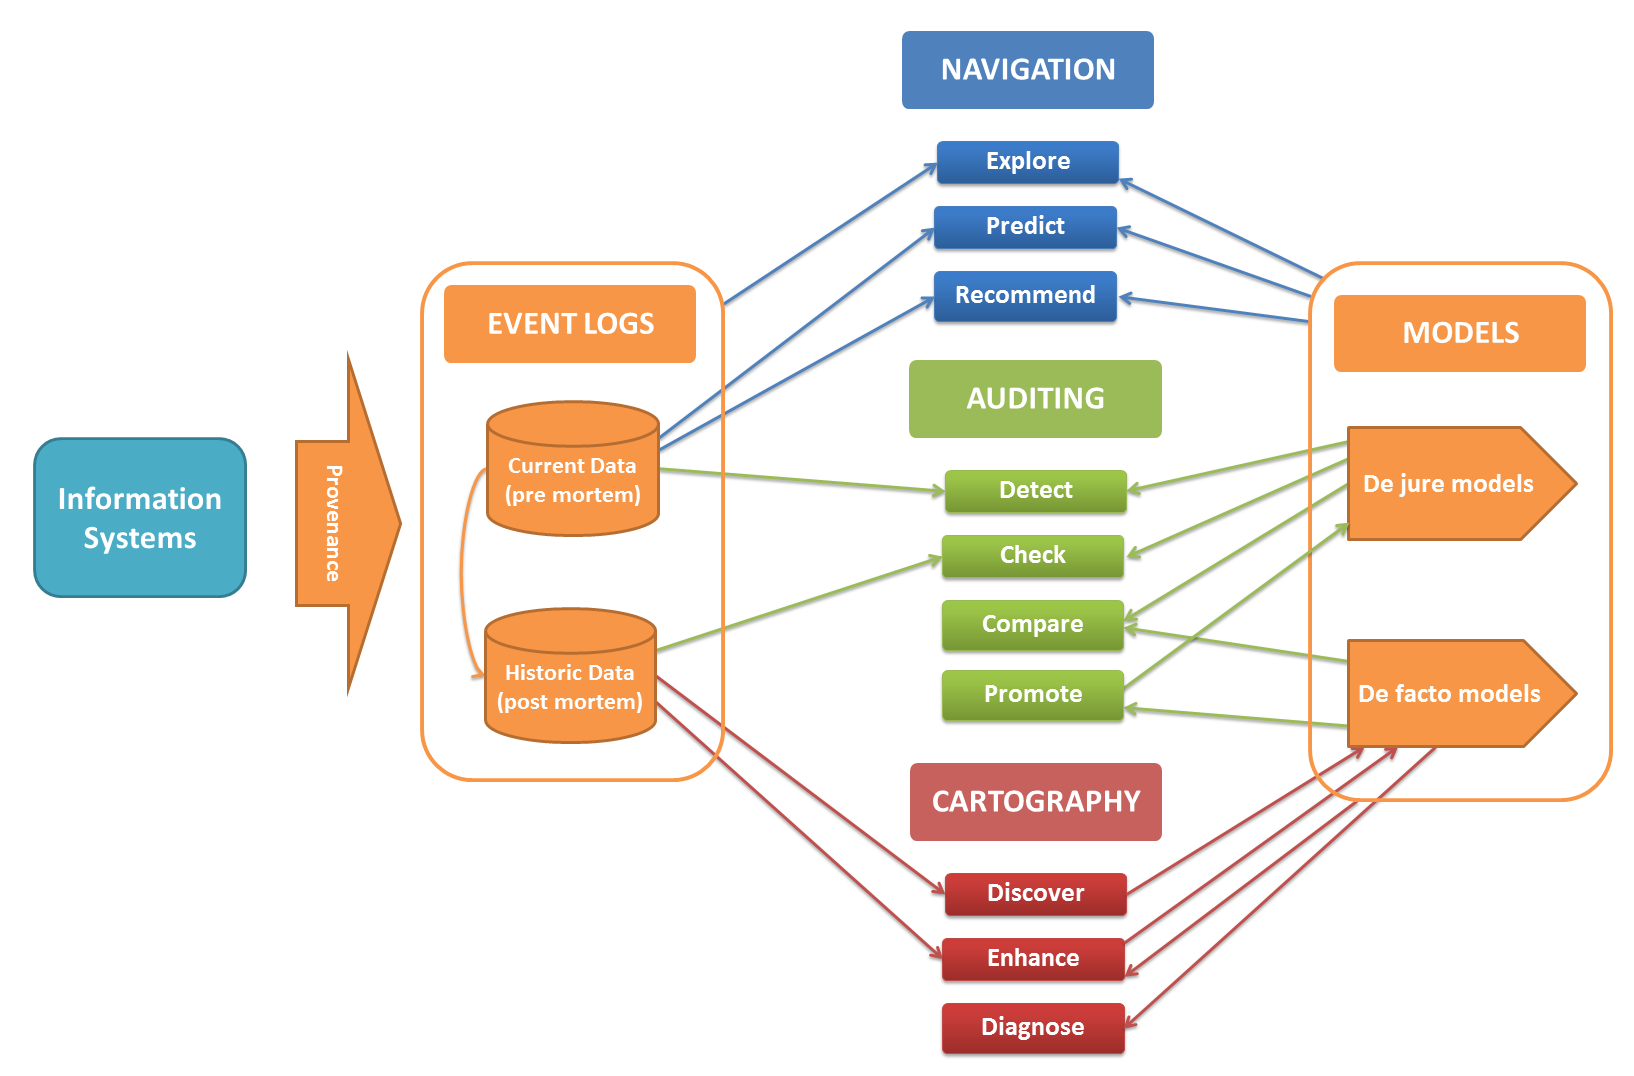
\includegraphics[width=\textwidth]{2_relatedwork/process-mining-spectrum-v2}
  \caption{Process Mining Framework}
  \label{fig:process-mining-spectrum-v2}
\end{figure}

Current challenges in the process mining area can be presented best through mentioning spectrum and its relations. As diagrammed in Figure~\ref{fig:process-mining-spectrum-v2} and presented in the research of van der Aalst \cite{van2011process}, process mining spectrum is extensive and highly inter-related. Starting with the provenance, process mining deals with gathering and keeping event logs as \textit{current data} and \textit{historic data}. In this level, \textit{post mortem data} means the logs and information gathered from completed events whereas \textit{pre mortem data} means information related to ongoing cases. This separation helps us to use historical knowledge to exploit and gain advantage over current business operations. At the very bottom of the diagram, models are presented as \textit{de facto models} and \textit{de jure models}. \textit{De jure models} are created with the aim of describing reality as it should be whereas \textit{de facto models} aims to describe reality as it is. Within each model category a mixture of perspectives, in other words point of views from different information levels, can be mixed. In order to fill the gap between event logs and models, ten different process mining activities are listed under three categories \cite{van2011process} as follows:
\begin{description}
\item[Cartography:] In this category the main aim is to create maps of the real world activities by using process models. 
	\begin{description}
	\item[Discovery:] Discovery is focused on extracting process models from event logs. 
	\item[Enhancing:] Enhancing activities are based on improving \textit{de facto models} with the information hidden in the event logs. 
	\item[Diagnose:] Diagnose activities stand for identifying the problems caused by directly process models.
	\end{description}
\item[Auditing:] In this category, activities related to confronting the model and the reality are collected.
	\begin{description}
	\item[Detect:] Detection is based on comparing the \textit{de jure models} with the ongoing processes to generate alerts if shifts occur in the reality.
	\item[Check:] Checking is defined to identify deviations occurred in the past.
	\item[Compare:] Comparison of \textit{de facto models} and \textit{de jure models} shows the difference between planned and the reality.
	\item[Promote:] Promotion includes  partially updating \textit{de jure models} from the information gathered from \textit{de facto models}.
	\end{description}
\item[Navigation:] In this category, process mining methods are used like a navigation application.
	\begin{description}
	\item[Explore:] Event data and models are used in combination to explore business processes.
	\item[Predict:] Prediction activities combine the information from past events and make predictions about ongoing processes.
	\item[Recommend:] Suitable actions can be suggested by using the prediction and contextual  information.
	\end{description}
\end{description}

Within this framework, the study presented in this thesis is a combination of discovery from cartography, promoting from auditing and recommendation from navigation. In other words and within the metaphor of spectrum, this study aims to discover maps using the discovery techniques and promotes the partially best locations in the map to create recommendations for travelers in their navigation applications. 

\section{Process Discovery in Process Mining}
\label{sec:process-discovery-in-process-mining} 
In this section, process discovery studies will be presented briefly. Within the process mining framework, there are various different process mining algorithms proposed which have the same aim of discovering underlying processes. Considering the approaches undertaken with the proposed algorithms, the following grouping is provided \cite{khodabandelou2013process}.

\begin{description}
\item[$\alpha$-algorithm:] This algorithm is based on the causality relationship that can be discovered from the event logs and proposed by van der Aalst et al. \cite{van2004workflow}. However, this approach cannot handle loops and extensions like $\alpha$++ algorithm \cite{de2004process} is proposed to overcome this problem. Discovery is focused on extracting process models from event logs. Outputs of this approaches are workflow nets with XOR, AND splits and joins to represent underlying process models.
\item[Inductive Approach:] Methods proposed in this approach \cite{herbst1998integrating} \cite{herbst2000dealing} is based on finding the best Hidden Markov Models (HMMs) that represents the underlying process model. Workflow nets are constructed by using HMM nodes and inductive learning.
\item[Hierarchical Clustering:] This method \cite{greco2005mining} firstly splits the event logs into clusters and creates a dependency graph. Using this dependency graph, clusters are defined with a hierarchy tree which is then merged into a single workflow model.
\item[Genetic Approach:] The method provided in this group \cite{van2005genetic} constructs models based on causal matrix of activities and tries to handle noise, incompleteness, concurrency, hidden and duplicate activities. However, there are many configuration parameters to handle noise and irrelevant data to use this methods. 
\item[Heuristic Approach:]Heuristic approach for process discovery is an extension of \alpha-algorithm which is based on likelihood calculation of activities and constructs dependency and frequency graphs. In addition, this method can handle noise in the event log and its implementation needs careful configuration.
\end{description}
 
Proposed methods in process discovery are based on solving different challenges in the process mining area. Considering the scope of this thesis study; process discovery operations are undertaken with inductive methods which is a robust, repeatable and mature set of approaches.

\section{Cross-organizational Process Mining}
\label{sec:cross-organizational-process-mining}
In this section, related studies and trends in cross-organizational process mining will be presented. Cross-organizational mining is based on cross-correlation of workflows and the realized activities in different organizations. The main challenge of this topic in process mining is that comparing processes and their performances of different organizational units in an objective approach. This objective approach is open to be enhanced with the process context, namely the environment of the process that is executed. Most of the studies in this area are currently studying to reveal the possible opportunities and some initial approaches to address main challenges.

In the study of Bujis et al. \cite{buijs2012towards}, the authors indicated the importance of the increase of Software-as-a-Service (SaaS) and cloud computing infrastructure usages. As a result of this increase, more and more organizations will use a Shared Business Process Management Infrastructure (SBPMI) and it is an opportunity for different organizational units to learn from each other in such infrastructure. The approach presented in this study is based on three questions and three metric groups to answer these questions:
\begin{enumerate}
\item Which organizations support my behavior with better process models?
\item Which organizations have better behavior which my process model supports? and
\item Which set of organizations can I support with my process model?
\end{enumerate} While answering these questions, they used \textit{simplification based metrics} to indicate better process models; and \textit{throughput time metrics} to indicate better behaviors. In this study, it is shown how a generic framework can be used to highlight the main idea behind cross-organizational process mining. 

In the study of van der Aalst \cite{van2011business}, using configurable process models is proposed for the organizations sharing the same infrastructure and doing the similar work. Configurable process models are defined as a family of process models where each organization can use this family with their configurations according to their business needs. This approach not only creates behaviors needed by each organization but also creates a basis to compare and learn within process mining framework. The configurable process models are formalized by "Causal Nets", which is a notational language based on input and output bindings of each node. Although this study does not answer to all challenges related to cross-organizational-process-mining, a formalism of configurable processes models is presented to address learning and conformance checking.

Cross-organizational process mining is divided into intra-organizational and inter-organizational with two basic ideas: \textit{collaboration} and \textit{exploiting} commonality \cite{van2011intra}. In his study, van der Aalst defined collaboration for distributed work between multiple organizations and commonality as ability of using same process models and infrastructure between the organizations. In order to exploit these two ideas, two partitioning dimensions are suggested in \cite{van2011intra}:
\begin{description}
	\item[Vertical Partitioning:] Process instances, namely cases, distributed over several organizations which collaborate to complete a complex activity. 
	\item[Horizontal Partitioning:] Process parts, namely tasks or activities, are shared within organizations like jigsaw puzzle parts.
\end{description}
For these orthogonal dimensions, a number of questions and challenges are presented in the study  \cite{van2011intra}. For the vertical partitioning, where organizations are aiming to share infrastructure and knowledge to learn from each other, it is mentioned that supervised learning methods like classification can be used. Notion of this thesis is based on vertical partitioning of cross-organizational process mining with the idea of unsupervised learning where predictor variables related to performances of organizations are used.
 
\section{Process Similarity in Process Mining}
\label{sec:process-similarity-in-process-mining}

In this section, prominent studies related to similarity in process mining will be presented with their results. With the emerging attention in business processes, organizations become aware of the fact that they can exploit the business processes and their similarities \cite{buijs2014comparing}. In addition, most of the large organizations have repository of process models of similar business operations \cite{dijkman2011similarity}. There are three main different approaches proposed to this solution in the literature currently. 

The first approach, proposed by Dijkman et al. \cite{dijkman2011similarity}, is based on similarity metrics as 
\begin{inparaenum}[\itshape a\upshape)]
\item node matching similarity;
\item structural similarity; and
\item behavioural similarity.
\end{inparaenum}
Result of the study \cite{dijkman2011similarity} indicates that using these three similarities can differentiate comparable process models and within these metrics structural similarity is the most prominent one. 

The second approach by Bujis and Reijis is an analytical approach \cite{buijs2014comparing} to compare the process models of different organizations that does similar works. Proposed algorithm is based on creating an alignment matrix between observed and realized models. This inter-relation is also used to compare different variants of the same process by different organizations. In addition, they suggested their method as a framework to further standardize a process of common interest. 

The third and final approach is based on frequently occurring mismatches between similar business processes \cite{dijkman2007mismatch}. In this study \cite{dijkman2007mismatch}, a set of mismatch patterns are derived from the different department of the same organization. Although this research does not present a complete set of possible mismatch patterns, the provided set is comprehensive to identify similarities and differences of the processes of same operations. In this thesis, combination of metric and mismatch pattern approaches are used to identify variations between process models of different organizations.

\section{Performance and Conformance Analysis in Process Mining}
\label{sec:performance-and-conformance-analysis-in-process-mining}
In this section summary of studies related to performance and conformance analysis will be presented. Event logs do not only contain task sequences but also contain time, resource and contextual information. Analysis of process models with these additional information is used within performance analysis framework to highlight bottlenecks or make predictions. However, in order to undertake a performance analysis there is a need of replaying reality (event logs) on the expectation (process models) and check the conformance of reality to plan \cite{van2012replaying}. 

In the study conducted by Rozinat and van der Aalst \cite{rozinat2008conformance}, a conformance framework is proposed by two metrics \textit{fitness metrics} and \textit{appropriateness metrics}. In this study \cite{rozinat2008conformance}, fitness metric is based on replaying the event log on the process model and counting the number of missing or remaining tokens. In other words, replaying and conformance of event logs over process models is modelled as a token passing formalism. On the other hand, appropriateness metrics are based on how accurate the process model in describing reality within a degree of clarity. Simplicity, precision and generalization attributes of the process models are taken into account while calculating appropriateness metrics.

Token passing approach to conformance has a major drawback when the process model and reality of event logs do not fit completely. In this case, there are overestimated process models that are too general, in other words with too much behavior other than the reality. In order to overcome this drawback, heuristic and optimization based methods are proposed by other researchers. In this thesis study, an extended version of optimization based approach presented in \cite{adriansyah2011conformance} is used to replay logs on the process models. Since the main goal of this study is not to evaluate conformance of logs and process models, the method presented by Adriansyah et al. is extended to calculate performance indicators while replaying the logs.